\section{Results}
\label{sec:results}

We first report how scores change relative to greedy (\secref{sec:res-scores}). We then test each hypothesis: reasoning (\secref{sec:res-reasoning}), ranking stability (\secref{sec:res-tau}), seed variability (\secref{sec:res-seed}), and creative writing (\secref{sec:res-creative}).

\begin{table}[t]
    \centering
    \resizebox{\textwidth}{!}{%
    \begin{tabular}{@{}lcccccc@{}}
        \toprule
        \textbf{Domain (unit)} & \greedy & \tsev & \tone & \topp & \topk & \minp \\
        \midrule
        Factual (acc.\ \%) & \textbf{51.8} & 50.2 {\scriptsize ($-$1.6\sig)} & 47.4 {\scriptsize ($-$4.3\sig)} & 49.0 {\scriptsize ($-$2.8\sig)} & 48.0 {\scriptsize ($-$3.8\sig)} & 50.2 {\scriptsize ($-$1.6\sig)} \\
        Reasoning (acc.\ \%) & \textbf{79.3} & 77.2 {\scriptsize ($-$2.0\pstar)} & 73.3 {\scriptsize ($-$5.9\sig)} & 76.3 {\scriptsize ($-$2.9\sig)} & 73.5 {\scriptsize ($-$5.7\sig)} & 76.7 {\scriptsize ($-$2.5\pstar)} \\
        Code (pass@1 \%) & \textbf{63.5} & 61.2 {\scriptsize ($-$2.3\pstar)} & 56.9 {\scriptsize ($-$6.7\sig)} & 60.6 {\scriptsize ($-$3.0\pstar)} & 56.6 {\scriptsize ($-$6.9\sig)} & 61.0 {\scriptsize ($-$2.5\pstar)} \\
        Creative (judge, 1--10) & 8.30 & 8.33 {\scriptsize ($+$0.03\pstar)} & 7.71 {\scriptsize ($-$0.59\sig)} & 8.30 {\scriptsize ($+$0.00\pstar)} & 8.30 {\scriptsize ($+$0.00\pstar)} & \textbf{8.35} {\scriptsize ($+$0.05\pstar)} \\
        \bottomrule
    \end{tabular}}
    \caption{Mean score over 11 models for each domain and strategy. The change relative to greedy is in parentheses. \sig: Wilcoxon signed-rank test over the 11 models, Holm-adjusted $p<0.05$ across all 20 tests. The best strategy in each row is in \textbf{bold}. Greedy is best in every verifiable domain. \tone and \topk lose the most, and \tsev, \topp, and \minp lose about half as much.}
    \label{tab:main}
\end{table}


\subsection{Sampling lowers accuracy in every verifiable domain}
\label{sec:res-scores}

\Tabref{tab:main} and \figref{fig:delta} show that greedy decoding gives the highest mean score in all three verifiable domains. No sampler beats it on average. The order of strategies is nearly the same in every domain: greedy $>$ \{\tsev, \minp, \topp\} $>$ \{\topk, \tone\}. \topk is almost indistinguishable from untruncated \tone. Factual QA drops 3.8 vs.\ 4.3 points, reasoning 5.7 vs.\ 5.9, and code 6.9 vs.\ 6.7. A fixed cut-off of 40 tokens rarely removes anything from the peaked distributions of instruction-tuned models. The adaptive samplers, top-$p$ and min-$p$, do remove the long tail and lose only 1.6--3.0 points.

\begin{figure}[t]
    \centering
    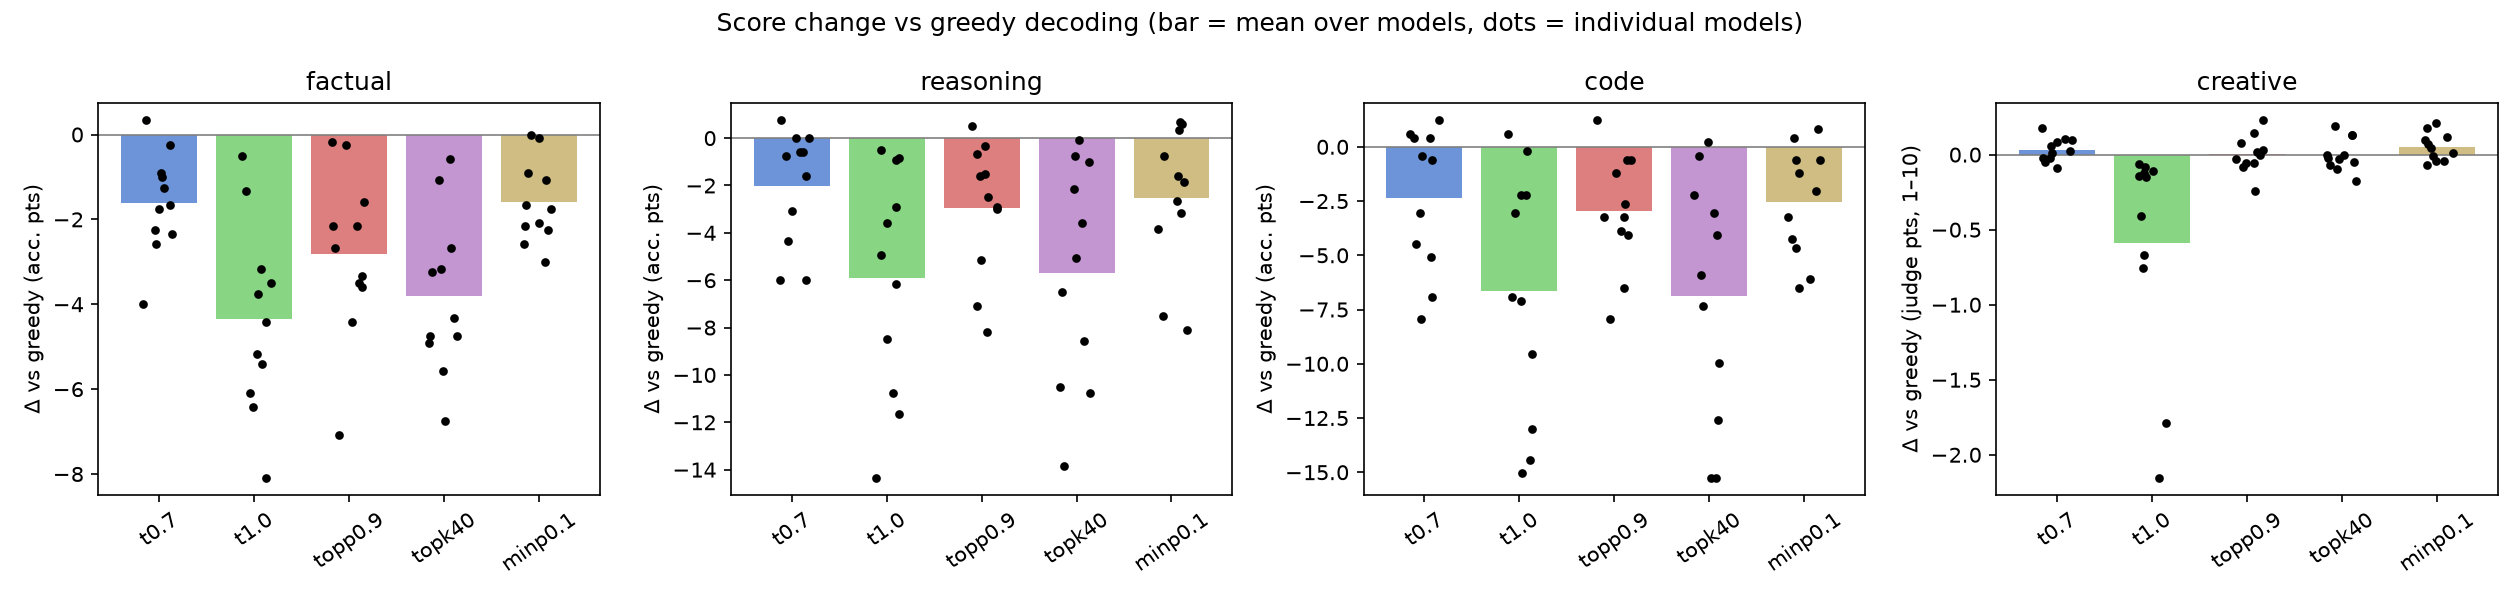
\includegraphics[width=0.98\linewidth]{figures/delta_vs_greedy.png}
    \caption{Change in score relative to greedy decoding for each domain and strategy. Bars show the mean over the 11 models, and dots show individual models. In the three verifiable domains, nearly every model loses accuracy under every sampler. Losses under \tone and \topk reach 8--15 points for some models. Creative quality is flat except at \tone.}
    \label{fig:delta}
\end{figure}

\para{H1: factual QA is not decoding-invariant (refuted).} All five samplers significantly reduce \triviaqa accuracy (Holm-adjusted $p\leq0.035$). The mean drop ranges from 1.6 points (\tsev, \minp) to 4.3 points (\tone), or 4.0--11.0\% in relative terms. Individual models lose up to 8.1 points. The 2-point bound in H1 holds only for the two mildest samplers, and only on average: under \tsev one model still loses 4.0 points. The item-level pattern explains why. Pooled over models, items that greedy answers correctly remain correct in only 87\% of \tone samples, while items that greedy gets wrong become correct in only 5\% of samples. Sampling mostly turns confident correct answers into plausible wrong ones and rarely rescues a miss. Relative to its lower base accuracy, factual QA loses about as much as reasoning (11.0\% vs.\ 8.6\% at \tone).

\subsection{The reasoning gap is real on average but model-dependent}
\label{sec:res-reasoning}

\begin{table}[t]
    \centering
    \small
    \begin{tabular}{@{}lcccc@{}}
        \toprule
        \textbf{Model} & \textbf{Greedy acc.} & \textbf{Gap: greedy $-$ \tone} & \textbf{\topp recovery} & \textbf{\minp recovery} \\
        \midrule
        Qwen2.5-0.5B & 50.5 & 14.3 & 51\% & 48\% \\
        Qwen2.5-1.5B & 72.5 & 11.7 & 74\% & 73\% \\
        Llama-3.1-8B & 85.0 & 10.8 & 52\% & 64\% \\
        Falcon3-7B & 87.0 & \phantom{0}8.5 & \phantom{0}4\% & \phantom{0}5\% \\
        Mistral-7B & 55.5 & \phantom{0}6.2 & 74\% & 57\% \\
        Phi-3-mini & 80.8 & \phantom{0}4.9 & 49\% & 63\% \\
        Qwen2.5-3B & 84.8 & \phantom{0}3.6 & 19\% & 56\% \\
        Olmo-3-7B & 88.0 & \phantom{0}2.9 & 49\% & 120\% \\
        Qwen2.5-7B & 89.2 & \phantom{0}0.9 & 155\% & 173\% \\
        Qwen3-4B & \textbf{90.8} & \phantom{0}0.8 & 60\% & 140\% \\
        Gemma-2-9B & 87.8 & \phantom{0}\textbf{0.5} & $-$33\% & $-$50\% \\
        \midrule
        Pooled & 79.3 & \phantom{0}5.9 & 50\% & 57\% \\
        \bottomrule
    \end{tabular}
    \caption{Per-model \gsm gap between greedy and \tone, and the share of that gap recovered by truncated sampling: $(\bar a_{\text{trunc}}-\bar a_{T=1})/(\bar a_{\text{greedy}}-\bar a_{T=1})$. Only 4 of 11 models fall in the hypothesized 5--12-point band. The gap shrinks as greedy accuracy rises, with Falcon3-7B as a notable exception. Recovery ratios are unstable when the gap is below about 1 point.}
    \label{tab:gap}
\end{table}


\para{H2 (mostly supported).} The mean \gsm gap between greedy and \tone is 5.9 points ($p_{\text{Holm}}=0.020$), inside the hypothesized 5--12-point band. \Tabref{tab:gap} shows that the per-model gap ranges from 0.5 to 14.3 points, and only 4 of 11 models fall inside the band. The gap shrinks as greedy accuracy rises. The three strongest reasoners (Qwen3-4B, Qwen2.5-7B, Gemma-2-9B, all above 87\% under greedy) lose less than 1 point. Small models lose 12--14 points. Falcon3-7B is an outlier: it is strong under greedy (87.0\%) but loses 8.5 points, and truncation hardly helps it. Pooled over models, \topp recovers 50\% of the \tone loss and \minp recovers 57\%. That meets the ``$>$50\%'' threshold only narrowly, so ``recovers most'' overstates it. Under \tsev and \minp, the reasoning loss is not significant after Holm correction ($p_{\text{Holm}}=0.13$ and $0.10$).

\begin{figure}[t]
    \centering
    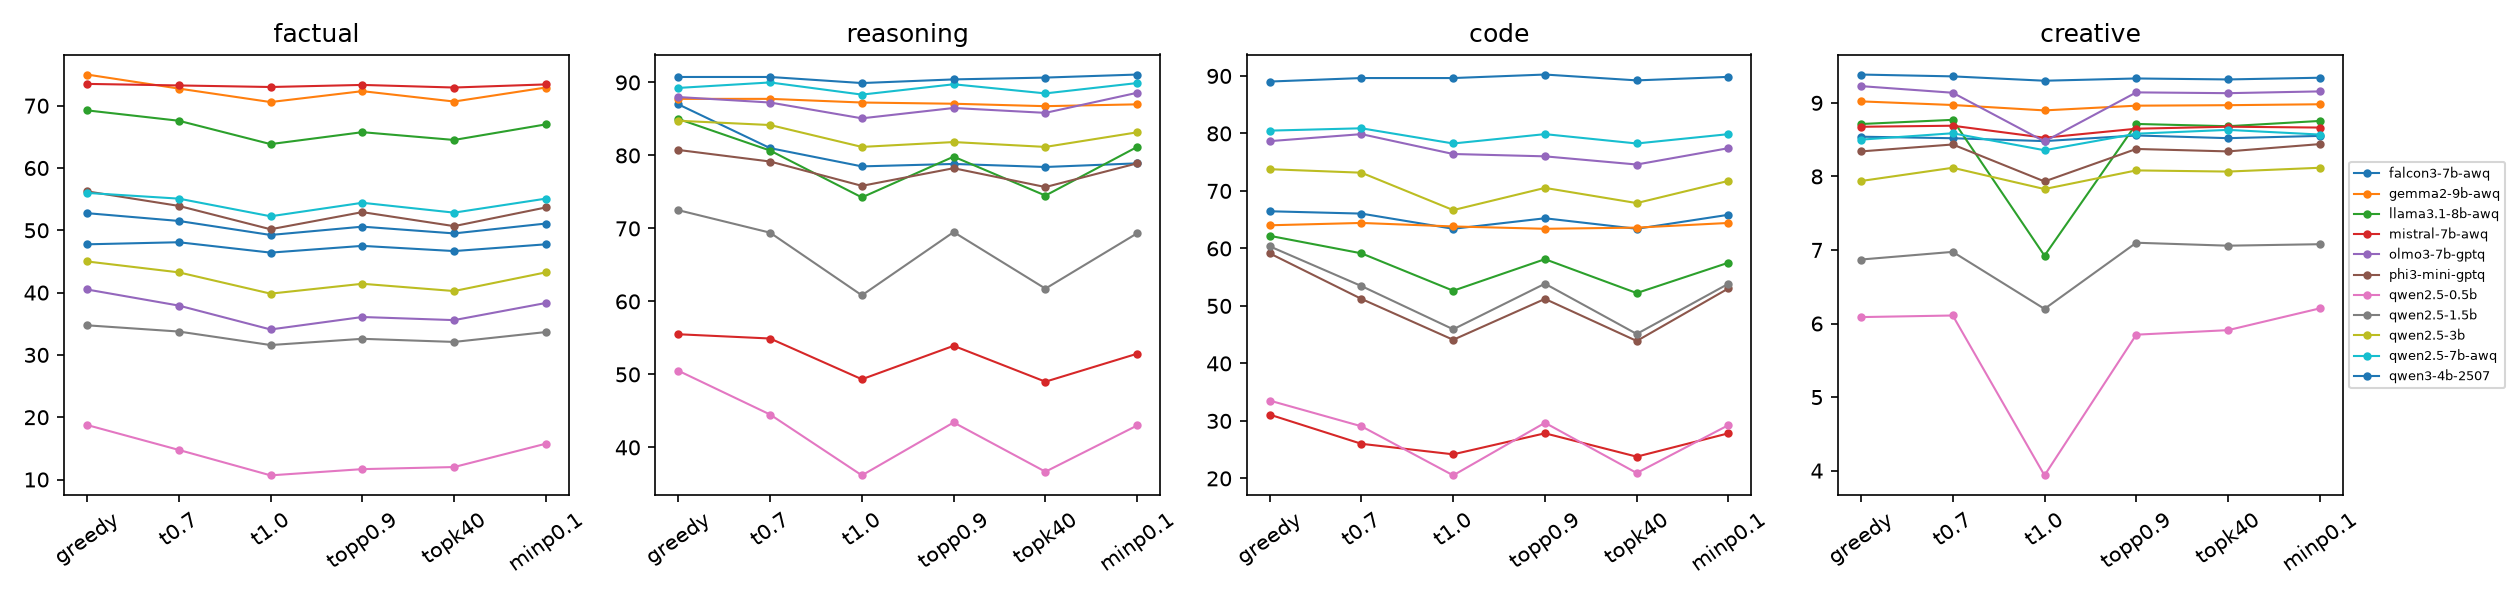
\includegraphics[width=0.98\linewidth]{figures/per_model_by_strategy.png}
    \caption{Per-model scores under each strategy. Most lines are nearly parallel, which is why rankings are stable. The visible V shapes at \tone and \topk come from weaker models (Qwen2.5-0.5B/1.5B, Phi-3-mini, Llama-3.1-8B). In the creative panel, Qwen2.5-0.5B and Llama-3.1-8B collapse only at untruncated \tone.}
    \label{fig:permodel}
\end{figure}

\subsection{Model rankings are stable; reasoning is the least stable verifiable domain}
\label{sec:res-tau}

\begin{table}[t]
    \centering
    \resizebox{\textwidth}{!}{%
    \begin{tabular}{@{}lcccccc@{}}
        \toprule
        & \multicolumn{5}{c}{\textbf{\ktau vs.\ greedy ranking [95\% item-bootstrap CI]}} & \\
        \cmidrule(lr){2-6}
        \textbf{Domain} & \tsev & \tone & \topp & \topk & \minp & \textbf{Mean pairwise $\tau$} \\
        \midrule
        Factual & 0.93 {\scriptsize [0.89, 1.00]} & 0.93 {\scriptsize [0.88, 1.00]} & 0.93 {\scriptsize [0.89, 1.00]} & 0.93 {\scriptsize [0.89, 1.00]} & 0.93 {\scriptsize [0.89, 1.00]} & \textbf{0.98} \\
        Reasoning & 0.89 {\scriptsize [0.71, 0.96]} & 0.85 {\scriptsize [0.71, 0.95]} & 0.85 {\scriptsize [0.70, 0.95]} & 0.85 {\scriptsize [0.71, 0.96]} & 0.85 {\scriptsize [0.70, 0.93]} & 0.91 \\
        Code & 1.00 {\scriptsize [0.80, 1.00]} & 0.93 {\scriptsize [0.76, 0.96]} & 1.00 {\scriptsize [0.80, 1.00]} & 0.93 {\scriptsize [0.77, 0.99]} & 1.00 {\scriptsize [0.80, 1.00]} & 0.96 \\
        Creative & 0.96 {\scriptsize [0.93, 1.00]} & 0.71 {\scriptsize [0.64, 0.81]} & 0.96 {\scriptsize [0.92, 1.00]} & 0.96 {\scriptsize [0.89, 1.00]} & 0.96 {\scriptsize [0.93, 1.00]} & 0.88 \\
        \bottomrule
    \end{tabular}}
    \caption{Ranking stability of the 11 models. The last column averages $\tau$ over all 15 pairs of strategies. The most stable domain overall is in \textbf{bold}. Every verifiable domain has $\tau\geq0.85$. The only value near 0.7 is creative writing at \tone, where small models degenerate.}
    \label{tab:tau}
\end{table}


\para{H4 (half supported).} \Tabref{tab:tau} and \figref{fig:tau} show that factual-QA rankings are stable: $\tau=0.93$ for every sampler (one swapped pair out of 55), and 85--97\% of bootstrap replicates exceed 0.9. As predicted, reasoning is the least stable verifiable domain, with $\tau$ between 0.85 and 0.89 and only 10--20\% of bootstrap replicates above 0.9. However, $\tau$ never comes close to the hypothesized $<0.7$. Point estimates are at least 0.85, and even the lower CI bounds are 0.70--0.71. The instability comes from tight clustering rather than from the domain itself. Under greedy, the top five \gsm models are within 3.75 points of each other (Qwen3-4B 90.8, Qwen2.5-7B 89.2, Olmo-3 88.0, Gemma-2 87.8, Falcon3 87.0), so small sampling effects swap neighbors. Code rankings are the most stable ($\tau=1.00$ under \tsev, \topp, and \minp), although their CIs are wide because \humaneval is small.

The only domain--strategy pair near $\tau=0.7$ is \emph{creative writing at \tone} ($\tau=0.71$ [0.64, 0.81]). Untruncated sampling makes some small models degenerate: Qwen2.5-0.5B loses 35\% of its judge score and Llama-3.1-8B loses 21\%, while Gemma-2-9B, Mistral-7B, Falcon3-7B, Qwen2.5-7B, and Qwen3-4B lose under 2\%. Stable rankings do not imply stable scores, however. Individual models move by up to 8.1 points on factual QA, 14.3 on reasoning, and 15.2 on code (\figref{fig:delta}), so comparing two models under different decoders can reverse the conclusion.

\begin{figure}[t]
    \centering
    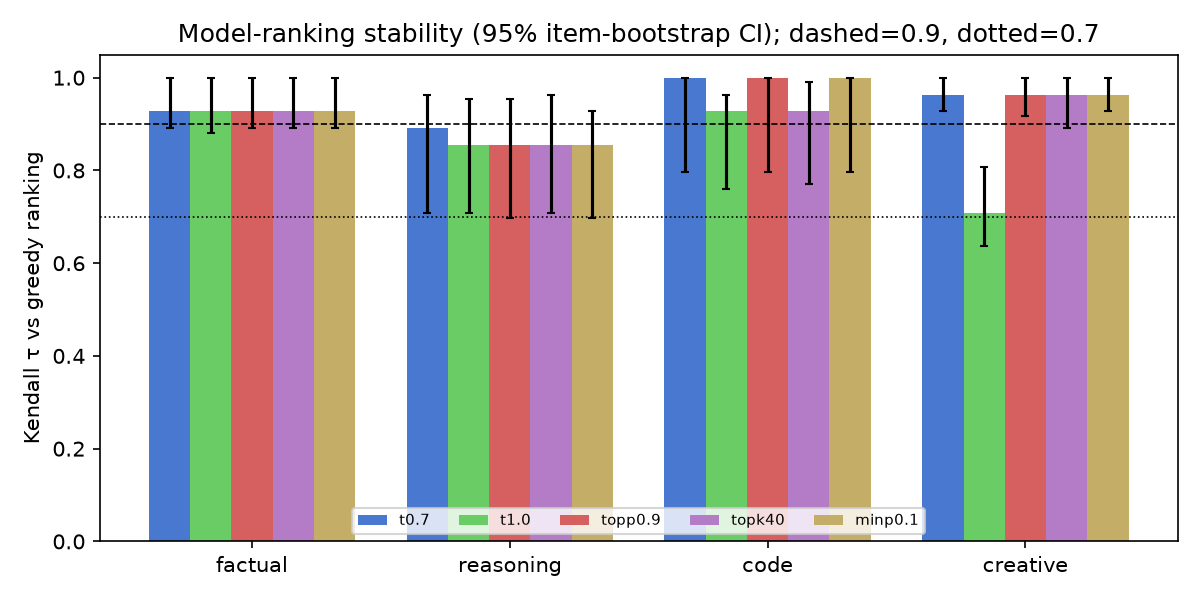
\includegraphics[width=0.7\linewidth]{figures/kendall_tau.png}
    \caption{\ktau between each strategy's model ranking and the greedy ranking, with 95\% item-bootstrap CIs. The dashed line marks 0.9 and the dotted line 0.7. Factual and code rankings stay near or above 0.9. Reasoning sits slightly lower (0.85--0.89) but well above 0.7. Only creative writing at \tone approaches 0.7.}
    \label{fig:tau}
\end{figure}

\subsection{Code is the most seed-sensitive domain}
\label{sec:res-seed}

\begin{table}[t]
    \centering
    \small
    \begin{tabular}{@{}lccccc@{}}
        \toprule
        \textbf{Domain} & \textbf{Items} & \textbf{Seed SD (pts)} & \textbf{Seed range (pts)} & \textbf{Item flip rate} & \textbf{SD / binomial SE} \\
        \midrule
        Code & 164 & \textbf{2.13} & \textbf{4.08} & \textbf{26.7\%} & \textbf{0.61} \\
        Reasoning & 400 & 1.16 & 2.21 & 24.2\% & 0.58 \\
        Factual & 398 & 1.14 & 2.18 & 14.4\% & 0.49 \\
        Creative (judge pts) & 100 & 0.05 & 0.09 & -- & -- \\
        \midrule
        \multicolumn{6}{@{}l}{\emph{Matched $n=164$ items (200 subsamples)}} \\
        Code & 164 & \textbf{2.13} & & & \\
        Reasoning & 164 & 1.85 {\scriptsize [1.61, 2.20]} & & & \\
        Factual & 164 & 1.59 {\scriptsize [1.30, 2.05]} & & & \\
        \bottomrule
    \end{tabular}
    \caption{Seed variability under sampling, averaged over 11 models $\times$ 5 sampled strategies. The flip rate is the share of items whose outcome differs across the 3 seeds. Code is the most seed-sensitive domain on every measure (paired Wilcoxon over 55 cells, $p<10^{-5}$; flip rate of code vs.\ reasoning, $p=0.02$). With matched $n$, code's lead over reasoning shrinks to 0.28 points.}
    \label{tab:seed}
\end{table}


\para{H5 (supported, with a caveat).} \Tabref{tab:seed} and \figref{fig:seed} show that code has the largest run-level seed SD (2.13 points, vs.\ 1.16 for reasoning and 1.14 for factual) and the highest item flip rate (26.7\%). More than a quarter of \humaneval problems change between pass and fail across seeds for the same model and sampler. These differences are significant (paired Wilcoxon over 55 cells, $p<10^{-5}$; $p=0.02$ for the flip rate of code vs.\ reasoning). Part of the raw gap comes from benchmark size. When \gsm and \triviaqa are subsampled to 164 items, their seed SD rises to 1.85 and 1.59, so code's lead over reasoning falls from 0.97 to 0.28 points. Normalized by the binomial standard error, code is still the highest (0.61 vs.\ 0.58 and 0.49). Creative judge scores average over 100 stories and many tokens, and they barely vary across seeds (SD 0.05 judge points).

\begin{figure}[t]
    \centering
    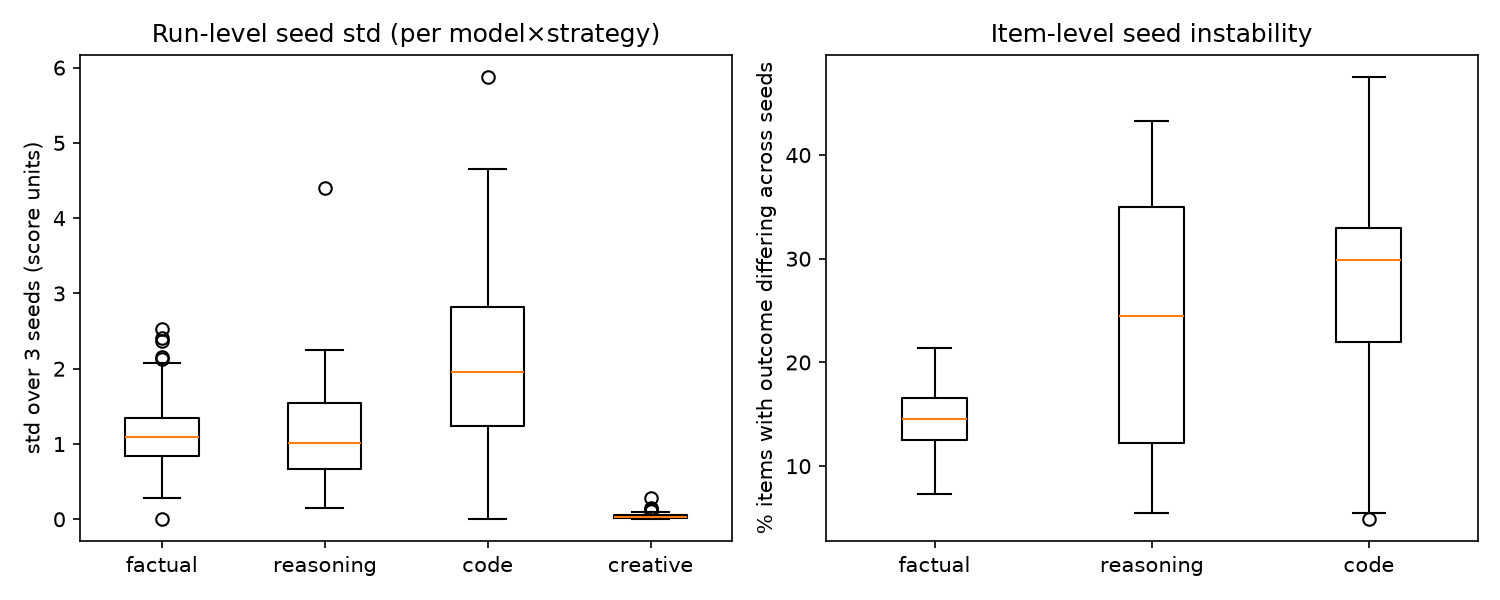
\includegraphics[width=0.85\linewidth]{figures/seed_variability.png}
    \caption{Seed variability by domain. \figleft Standard deviation of run-level scores over 3 seeds for each model$\times$strategy cell. \figright Share of items whose outcome differs across seeds. Code has the highest median and the widest spread on both measures. Reasoning flip rates vary widely across models.}
    \label{fig:seed}
\end{figure}

\subsection{Sampling does not improve judged creative quality}
\label{sec:res-creative}

\begin{table}[t]
    \centering
    \resizebox{\textwidth}{!}{%
    \begin{tabular}{@{}lcccccccc@{}}
        \toprule
        & \multicolumn{5}{c}{\textbf{LLM judge (1--10)}} & \multicolumn{3}{c}{\textbf{Surface statistics}} \\
        \cmidrule(lr){2-6} \cmidrule(lr){7-9}
        \textbf{Strategy} & Creativity & Coherence & Fluency & Engagement & Mean & Distinct-2 & Words & Truncated \\
        \midrule
        \greedy & 7.24 & \textbf{8.36} & \textbf{9.47} & 8.13 & 8.30 & 0.963 & 148 & \textbf{1.6\%} \\
        \tsev & 7.39 & 8.31 & 9.44 & 8.20 & 8.33 & 0.973 & 151 & 1.8\% \\
        \tone & 7.29 & 7.37 & 8.56 & 7.64 & 7.71 & \textbf{0.982} & 156 & 4.5\% \\
        \topp & 7.47 & 8.20 & 9.34 & 8.20 & 8.30 & 0.977 & 154 & 2.8\% \\
        \topk & \textbf{7.53} & 8.15 & 9.31 & \textbf{8.22} & 8.30 & 0.979 & 156 & 2.7\% \\
        \minp & 7.39 & 8.35 & 9.46 & 8.21 & \textbf{8.35} & 0.973 & 153 & 2.0\% \\
        \bottomrule
    \end{tabular}}
    \caption{Creative writing, averaged over 11 models. Sampling raises creativity (+2 to +4\%) and lexical diversity but lowers coherence and fluency, so the overall judge score stays flat or drops. \textbf{Bold} marks the best value per column, counting lower truncation as better.}
    \label{tab:creative}
\end{table}


\para{H3 (refuted).} Relative to greedy, the overall judge score changes by $+0.5\%$ (\tsev), $+0.0\%$ (\topp), $+0.0\%$ (\topk), and $+0.7\%$ (\minp), none of them significant. It falls by $7.9\%$ under \tone ($p_{\text{Holm}}=0.020$). None of these comes close to the hypothesized $+10$--$15\%$. \Tabref{tab:creative} shows why. Sampling does raise the judge's \emph{creativity} sub-score (by 2--4\%) and distinct-2 (from 0.963 to 0.973--0.982), but it lowers coherence and fluency by about the same amount. Greedy stories from instruction-tuned models are already fluent and coherent. Untruncated sampling visibly breaks small models: Qwen2.5-0.5B drifts into word salad (``Dory's repertoire of species expert claim proved invaluable\ldots''), and 27\% of its \tone stories hit the length cap.
